\textbf{COLUNI 2026 -- Questão 23}\par\medskip A radiação é o processo de propagação de calor por meio de ondas eletromagnéticas. O que diferencia um tipo de onda eletromagnética da outra é sua frequência ($f$) e seu comprimento de onda ($\lambda$). A velocidade de propagação ($v$) da onda eletromagnética é definida por $v=\lambda\cdot f$. A radiação oriunda do Sol que atinge a atmosfera é constituída de diversos comprimentos de onda. Os corpos ao serem aquecidos por esta radiação reemitem principalmente os comprimentos de onda maiores, referentes ao infravermelho. Quando a radiação é reemitida, a atmosfera reflete principalmente as ondas infravermelhas e promove o efeito estufa de aquecimento. A figura a seguir ilustra a situação de ondas eletromagnéticas provenientes do Sol, que ao penetrarem numa estufa retêm alguns comprimentos de ondas. De forma análoga, o aumento do gás carbônico na atmosfera promove o aquecimento global.

\begin{figure}[htbp]
\centering
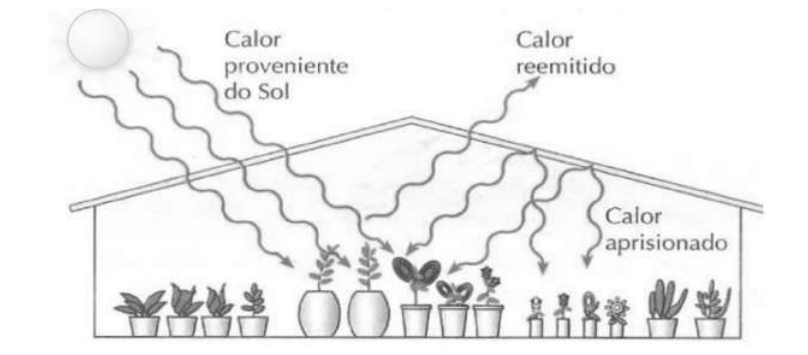
\includegraphics[width=0.78\linewidth]{static/simulados/coluni/figuras/2026/questao-23/figura-1.png}
\end{figure}

Disponível em: https://elysios.com.br/blog/a-dinamica-do-microclima-em-ambientes-protegidos/. Acesso em: 18 ago. 2025.

Das alternativas a seguir, a que explica o aquecimento global causado pelo efeito estufa, CORRETAMENTE, é:\begin{enumerate}
\item As radiações mais refletidas pela atmosfera são as que têm menores frequências.
\item As radiações mais refletidas pela atmosfera são as que têm maiores frequências.
\item Todas as radiações reemitidas pelos corpos presentes na atmosfera são refletidas.
\item Todas as radiações que chegam à atmosfera são absorvidas e nada é refletido.\end{enumerate}